\documentclass[aspectratio=169,xcolor=dvipsnames]{beamer}

% 1. Definir el color ANTES de llamar al tema SimplePlus
\usepackage{xcolor}
\definecolor{nyugray}{RGB}{128,128,128}

\usetheme{SimplePlus}
\definecolor{UnalGreen}{RGB}{0,153,51}
\usepackage[utf8]{inputenc}
\usepackage[spanish]{babel}
\usepackage{hyperref}
\usepackage{graphicx}
\usepackage{booktabs}
\usepackage{tikz}
\usetikzlibrary{positioning, arrows.meta}
\usepackage[skip=5pt]{caption}

\captionsetup{justification=justified, font=small}
\usefonttheme{professionalfonts}

% ----- INFORMACIÓN DE LA PRESENTACIÓN -----
\title{Fundamentos de Mecánica -- Taller (14)}
\subtitle{Sesión 1: Presentación del Curso, Unidades y Vectores}

\titlegraphic{%
    \vspace*{-0.3cm}%
    \IfFileExists{imagenes/universidad-nacional-de-colombia-sede-bogota-seeklogo.png}{%
        
\includegraphics[width=2.2cm]{imagenes/universidad-nacional-de-colombia-sede-bogota-seeklogo.png}%
    }{%
        \IfFileExists{universidad-nacional-de-colombia-sede-bogota-seeklogo.png}{%
            
\includegraphics[width=2.2cm]{universidad-nacional-de-colombia-sede-bogota-seeklogo.png}%
        }{}%
    }%
    \hspace{1.0cm}%
    % Logo MIAI
    \IfFileExists{logoMIAI_white.png}{%
        
\includegraphics[width=4.0cm]{logoMIAI_white.png}%
    }{%
        \IfFileExists{imagenes/logoMIAI_white.png}{%
            
\includegraphics[width=4.0cm]{imagenes/logoMIAI_white.png}%
        }{}%
    }%
}

\author{Miguel Andrés Perdomo Gutiérrez}

\institute{%
    Auxiliar Docente | M.Sc. en Ciencias -- Física\\
    Universidad Nacional de Colombia -- Sede Bogotá
}

\date{28 de agosto de 2026}

\begin{document}
    
    % ----- SLIDE 1: PORTADA -----
    \begin{frame}
        \titlepage
    \end{frame}
    
    % ----- SLIDE 2: INFORMACIÓN GENERAL -----
    \begin{frame}[shrink=5]{Información General}
        \begin{columns}[t]
            \begin{column}{0.48\textwidth}
                \textbf{Docente:}
                \begin{itemize}
                    \item Miguel Andrés Perdomo G.
                    \item \href{mailto:mperdomog@unal.edu.co}{\footnotesize mperdomog@unal.edu.co}
                \end{itemize}
                
                \vspace{0.15cm}
                \textbf{Horario y Lugar:}
                \begin{itemize}
                    \item Viernes 09:00--11:00
                    \item Edificio 401, Salón 202
                \end{itemize}
            \end{column}
            
            \begin{column}{0.48\textwidth}
                \textbf{Atención a Estudiantes:}
                \begin{itemize}
                    \item Cita previa por correo electrónico
                    \item Of. 2056 (G. Física Nuclear, Ed. Ancízar)
                \end{itemize}
                
                \vspace{0.15cm}
                \textbf{Equipos de Trabajo:}
                \begin{itemize}
                    \item Grupos fijos de \textbf{4 integrantes}.
                \end{itemize}
            \end{column}
        \end{columns}
        
        \vspace{0.2cm}
        
        \begin{center}
            \IfFileExists{Images/map2.png}{%
                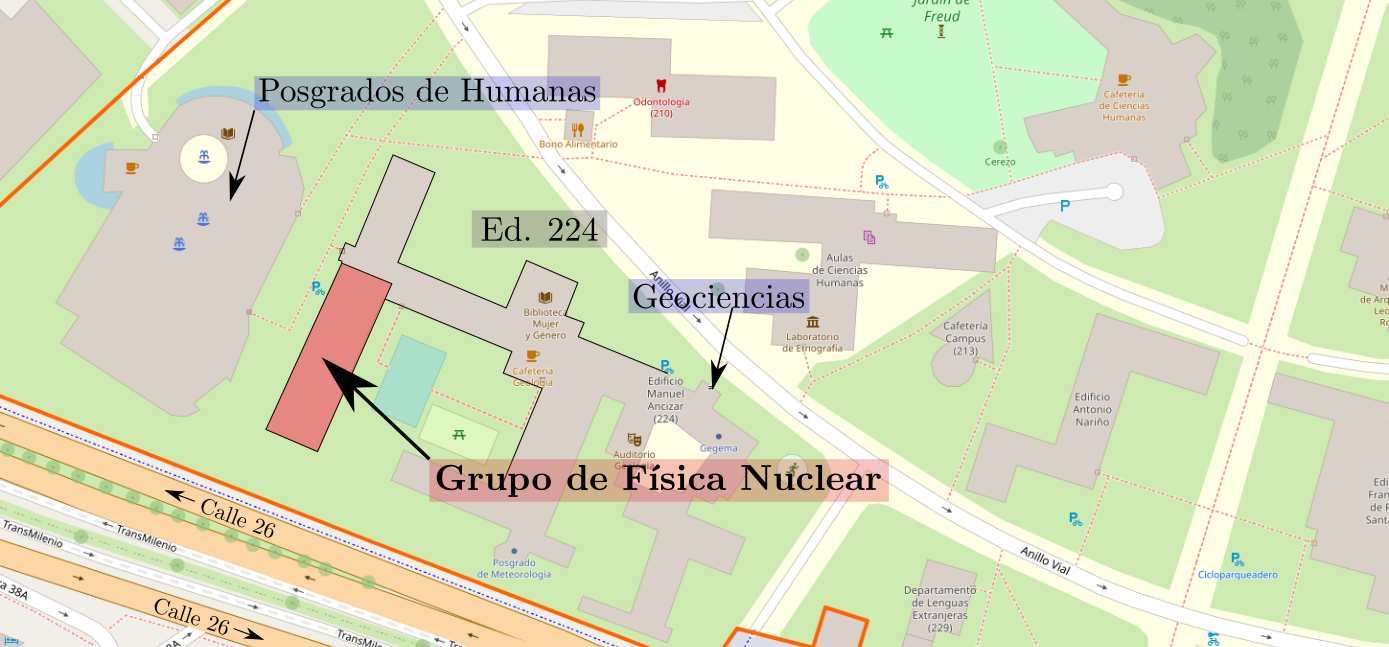
\includegraphics[height=4.2cm, keepaspectratio]{Images/map2.png}%
            }{%
                \IfFileExists{imagenes/map2.png}{%
                    
\includegraphics[height=4.2cm, keepaspectratio]{imagenes/map2.png}%
                }{%
                    \small \textit{[Ubicación Edificio 401 y Oficina 2056]}%
                }%
            }
        \end{center}
    \end{frame}

    % ----- SLIDE 3: OBJETIVOS Y ROL DEL TALLER -----
% ----- SLIDE 3: OBJETIVOS Y ROL DEL TALLER -----
\begin{frame}{Objetivos del Taller}
	\begin{columns}[T]
		% ----- ÍCONO 1: PRÁCTICA -----
		\begin{column}{0.3\textwidth}
			\centering
			\begin{tikzpicture}[scale=0.75]
			% Tablero / Clipboard
			\draw[fill=UnalGreen!12, draw=UnalGreen, thick, rounded corners=4pt] (-1,-1.2) rectangle (1,1.2);
			\draw[fill=UnalGreen, draw=UnalGreen, rounded corners=1pt] (-0.35,1.1) rectangle (0.35,1.35);
			% Renglones / Fórmulas
			\draw[thick, UnalGreen!80!black] (-0.6,0.6) -- (0.6,0.6);
			\draw[thick, UnalGreen!80!black] (-0.6,0.2) -- (0.2,0.2);
			\draw[thick, UnalGreen!80!black] (-0.6,-0.2) -- (0.5,-0.2);
			% Chulo / Checkmark
			\draw[ultra thick, UnalGreen] (-0.4,-0.7) -- (-0.1,-0.95) -- (0.6,-0.5);
			\end{tikzpicture}
			
			\vspace{0.2cm}
			\textbf{Práctica}
		\end{column}
		
		% ----- ÍCONO 2: COLABORACIÓN -----
		\begin{column}{0.3\textwidth}
			\centering
			\begin{tikzpicture}[scale=0.75]
			% Usuario central
			\fill[UnalGreen] (0,0.4) circle (0.35);
			\fill[UnalGreen] (-0.55,-0.7) arc (180:0:0.55) -- cycle;
			% Usuario izquierdo
			\fill[UnalGreen!50] (-0.75,0.2) circle (0.28);
			\fill[UnalGreen!50] (-1.2,-0.7) arc (180:0:0.45) -- cycle;
			% Usuario derecho
			\fill[UnalGreen!50] (0.75,0.2) circle (0.28);
			\fill[UnalGreen!50] (0.3,-0.7) arc (180:0:0.45) -- cycle;
			\end{tikzpicture}
			
			\vspace{0.2cm}
			\textbf{Colaboración}
		\end{column}
		
		% ----- ÍCONO 3: ARGUMENTACIÓN -----
		\begin{column}{0.3\textwidth}
			\centering
			\begin{tikzpicture}[scale=0.75]
			% Tablero de exposición
			\draw[fill=UnalGreen!12, draw=UnalGreen, thick, rounded corners=3pt] (-1.1,-0.3) rectangle (1.1,1.1);
			\draw[thick, UnalGreen] (-0.5,-0.3) -- (-0.75,-1.0);
			\draw[thick, UnalGreen] (0.5,-0.3) -- (0.75,-1.0);
			% Gráfica / Ideas en el tablero
			\draw[ultra thick, UnalGreen, ->] (-0.8,-0.0) -- (-0.8,0.8);
			\draw[ultra thick, UnalGreen, ->] (-0.8,-0.0) -- (0.8,-0.0);
			\draw[thick, UnalGreen!80!black] (-0.7,0.1) -- (-0.2,0.6) -- (0.2,0.3) -- (0.7,0.8);
			\fill[UnalGreen] (0.7,0.8) circle (0.06);
			\end{tikzpicture}
			
			\vspace{0.2cm}
			\textbf{Argumentación}
		\end{column}
	\end{columns}
	
	\vspace{0.5cm}
	
	\begin{block}{}
		\centering
		Afianzar conceptos mediante resolución de problemas, trabajo en equipo y sustentación en tablero.
	\end{block}
\end{frame}
    
    % ----- SLIDE 4: ESTRUCTURA DE LA SESIÓN -----
% ----- SLIDE 4: ESTRUCTURA DE LA SESIÓN -----
\begin{frame}{Estructura de la Sesión}
	\begin{center}
		\begin{tikzpicture}[node distance=0.8cm, auto]
		\node[rectangle, draw, fill=blue!10, rounded corners, text width=3cm, align=center] (org) {Organización\\\small 10 min};
		\node[rectangle, draw, fill=green!10, rounded corners, text width=3cm, align=center, right=of org] (tab) {Tablero\\\small 80 min};
		\node[rectangle, draw, fill=orange!10, rounded corners, text width=3cm, align=center, right=of tab] (eval) {Evaluación\\\small 20 min};
		\node[rectangle, draw, fill=red!10, rounded corners, text width=3cm, align=center, below=of tab] (pautas) {Pautas\\\small 10 min};
		
		\draw[->] (org) -- (tab);
		\draw[->] (tab) -- (eval);
		\draw[->] (tab) -- (pautas);
		\end{tikzpicture}
	\end{center}
\end{frame}
    
    % ----- SLIDE 5: SISTEMA DE EVALUACIÓN -----
\begin{frame}{Evaluación (sugerencia)}
	\begin{columns}[T]
		\begin{column}{0.48\textwidth}
			\centering
			\textbf{50\%}\\ Trabajo en Equipo
			\begin{itemize}
				\item Sustentación en tablero
				\item Memoria escrita
			\end{itemize}
		\end{column}
		\begin{column}{0.48\textwidth}
			\centering
			\textbf{50\%}\\ Evaluación Individual
			\begin{itemize}
				\item Quices quincenales
				\item Conceptos clave
			\end{itemize}
		\end{column}
	\end{columns}
	
	\vspace{0.3cm}
	\begin{alertblock}{}
		Preparación previa indispensable.
	\end{alertblock}
\end{frame}

    % ----- SLIDE 6: BIBLIOGRAFÍA Y RECURSOS -----
\begin{frame}{Bibliografía}
	\begin{itemize}
		\item[1] H. Young, H.D. Young, and R.A. Freedman, \textit{University Physics with Modern Physics}, 15th ed., Pearson, 2019.
		\vspace{0.15cm}
		\item[2] P. A. Tipler and G. Mosca, \textit{Physics for Scientists and Engineers with Modern Physics}, 6th ed., W. H. Freeman and Company, 2020.
		\vspace{0.15cm}
		\item[3] R. A. Serway and J. W. Jewett, \textit{Physics for Scientists and Engineers with Modern Physics}, 10th ed., Brooks Cole / Cengage Learning, 2019.
	\end{itemize}
	
	\vspace{0.4cm}
	\begin{block}{Canal Digital del Curso}
		El seguimiento del cronograma, guías de taller y material complementario estará disponible a través de la plataforma Google Classroom.
	\end{block}
\end{frame}

% ============================================================
% SLIDE: PREGUNTA INICIAL
% ============================================================
\begin{frame}{¿Alguien ha jugado canicas?}
	\begin{center}
		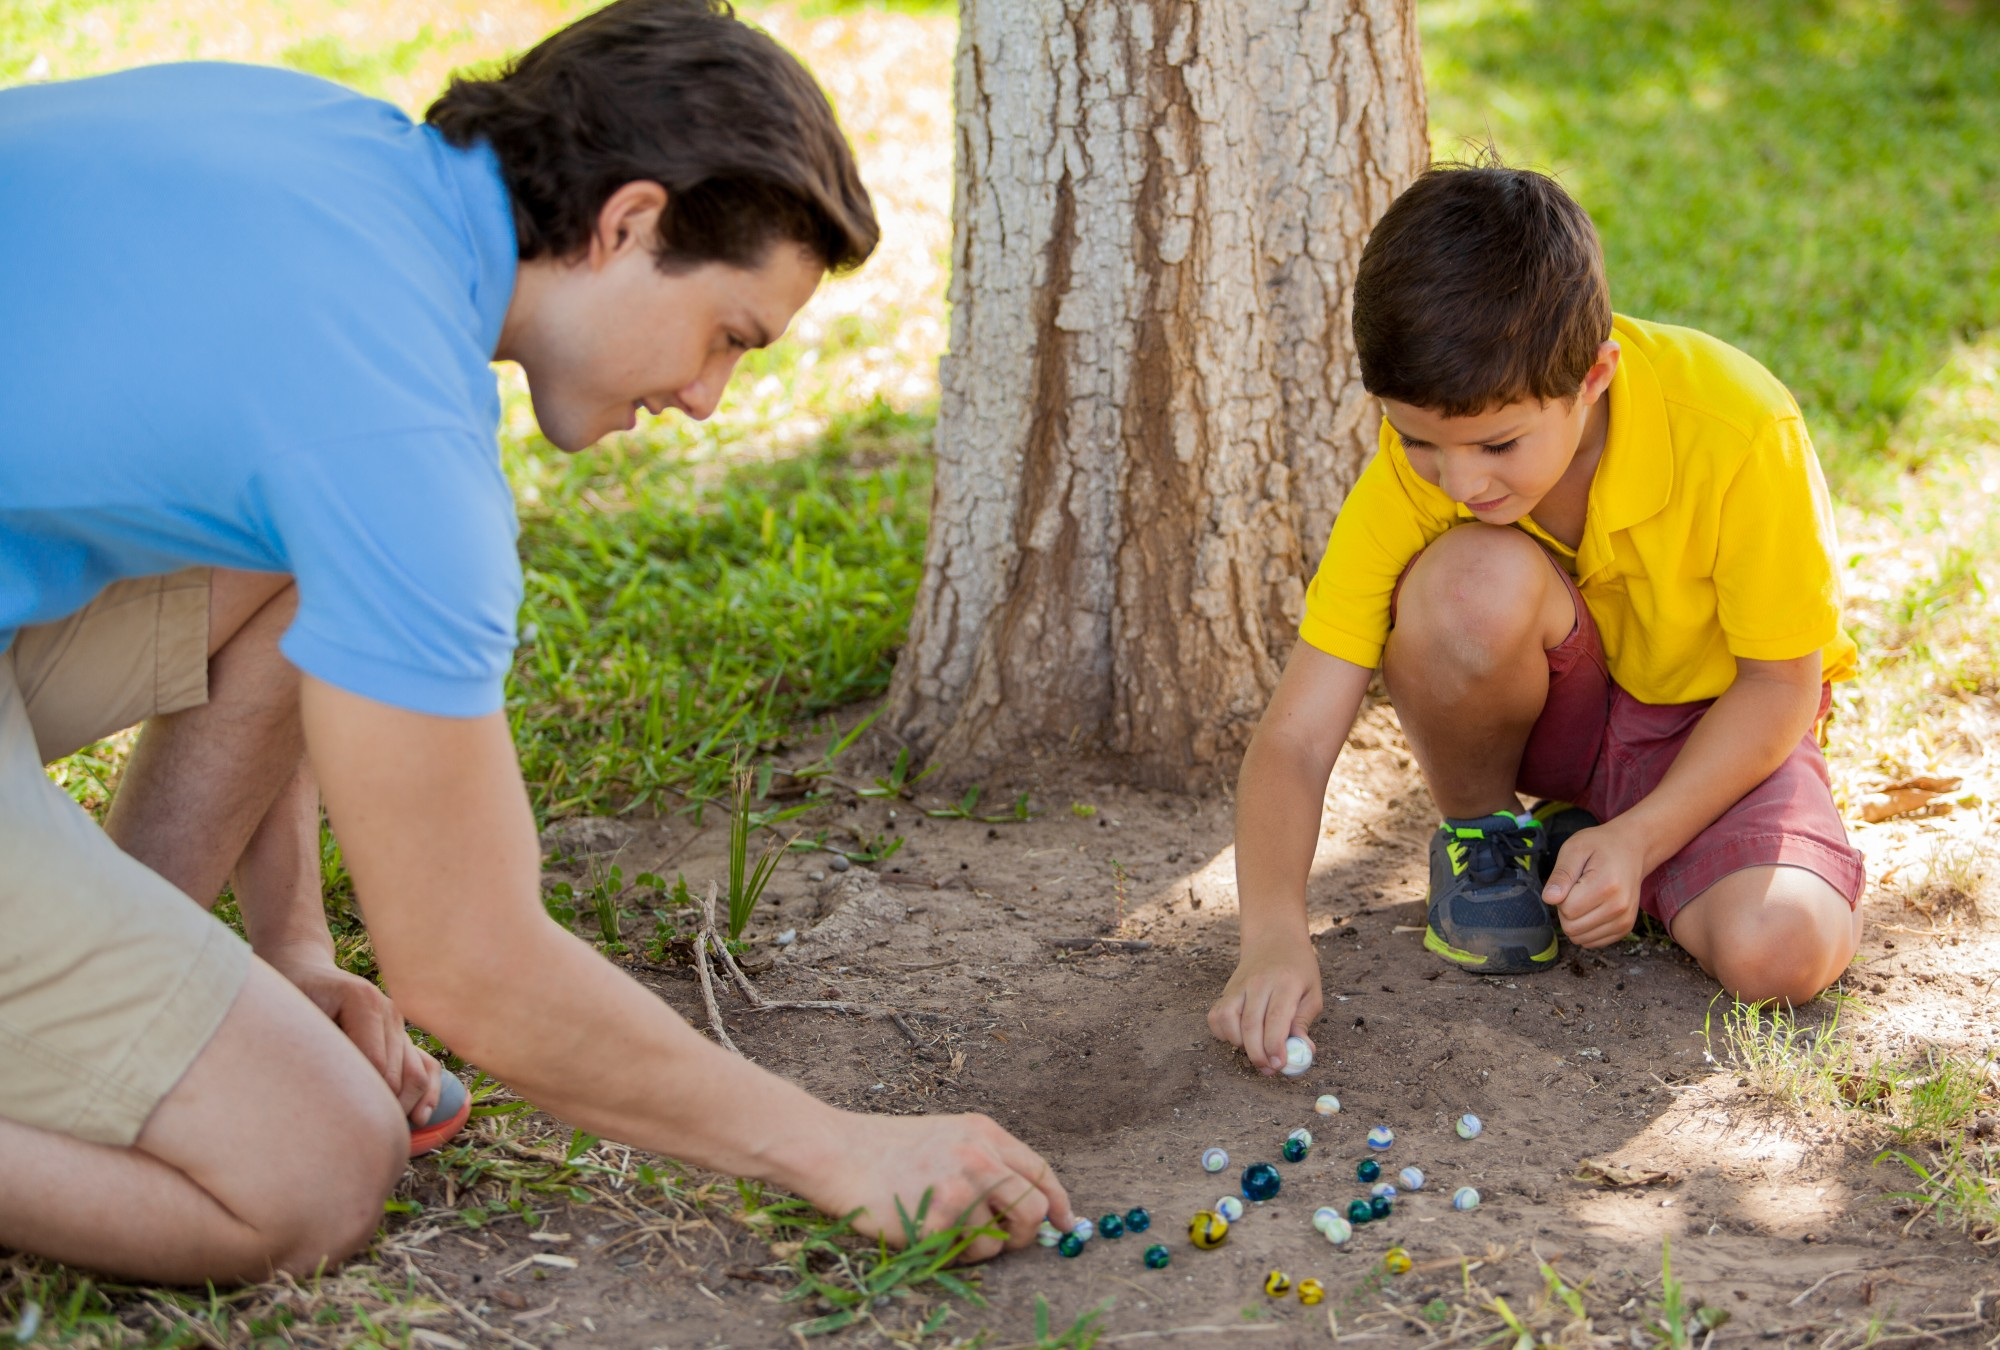
\includegraphics[width=0.4\textwidth]{Images/canicas-juegos.jpg} % imagen de canicas
	\end{center}
	
	\vspace{0.3cm}
	\begin{block}{}
		\centering
		¿Cómo se mide para eliminar al rival?
	\end{block}
	
	\vspace{0.2cm}
	\begin{itemize}
		\item \textbf{Medir} = comparar una magnitud desconocida con un \alert{patrón de referencia}.
		\item Ese patrón lo define el \textbf{SI}.
	\end{itemize}
\end{frame}


% ============================================================
% SLIDE: EL METRO
% ============================================================
\begin{frame}{El Metro}
	\begin{block}{Definición original (1791)}
		\centering
		Una diezmillonésima parte del cuadrante del meridiano terrestre.
	\end{block}
	
	\vspace{0.3cm}
	\begin{columns}[T]
		\begin{column}{0.48\textwidth}
			\textbf{Prototipo:}
			\begin{itemize}
				\item Barra de platino-iridio
				\item Museo de Sevres, París
			\end{itemize}
		\end{column}
		\begin{column}{0.48\textwidth}
			\textbf{Definición actual (1983):}
			\begin{itemize}
				\item Distancia que recorre la luz en $1/299\,792\,458$ s
			\end{itemize}
		\end{column}
	\end{columns}
\end{frame}


% ============================================================
% SLIDE: PREFIJOS Y NOTACIÓN CIENTÍFICA
% ============================================================
\begin{frame}{Prefijos y Notación Científica}
	\begin{columns}[T]
		\begin{column}{0.48\textwidth}
			\textbf{Prefijos comunes:}
			\begin{table}
				\small
				\begin{tabular}{c|c}
					\textbf{Prefijo} & \textbf{Factor} \\
					\hline
					pico (p) & $10^{-12}$ \\
					nano (n) & $10^{-9}$ \\
					micro ($\mu$) & $10^{-6}$ \\
					mili (m) & $10^{-3}$ \\
					centi (c) & $10^{-2}$ \\
					kilo (k) & $10^3$ \\
					mega (M) & $10^6$ \\
					giga (G) & $10^9$
				\end{tabular}
			\end{table}
		\end{column}
		\begin{column}{0.48\textwidth}
			\textbf{Ejemplos:}
			\begin{itemize}
				\item Radio del H: $0.529 \times 10^{-10}$ m = \alert{0.529 \AA}
				\item Radio del protón: $0.84 \times 10^{-15}$ m = \alert{0.84 fm}
				\item Distancia Tierra-Sol: $1.5 \times 10^{11}$ m
			\end{itemize}
		\end{column}
	\end{columns}
\end{frame}


% ============================================================
% SLIDE: MAGNITUDES FUNDAMENTALES Y DERIVADAS
% ============================================================
\begin{frame}{Magnitudes Físicas}
	\begin{columns}[T]
		\begin{column}{0.48\textwidth}
			\textbf{Fundamentales (7):}
			\begin{itemize}
				\item Longitud (m)
				\item Masa (kg)
				\item Tiempo (s)
				\item Corriente (A)
				\item Temperatura (K)
				\item Cantidad de sustancia (mol)
				\item Intensidad luminosa (cd)
			\end{itemize}
		\end{column}
		\begin{column}{0.48\textwidth}
			\textbf{Derivadas:}
			\begin{itemize}
				\item Velocidad: m/s
				\item Aceleración: m/s$^2$
				\item Fuerza: kg$\cdot$m/s$^2$ = N
				\item \textbf{Energía:} kg$\cdot$m$^2$/s$^2$ = J
			\end{itemize}
		\end{column}
	\end{columns}
	
	\vspace{0.2cm}
	\begin{exampleblock}{Análisis Dimensional}
		$E = \frac{1}{2}mv^2 $ \checkmark
	\end{exampleblock}
\end{frame}


% ============================================================
% SLIDE: VECTORES Y ESCALARES
% ============================================================
\begin{frame}{Vectores vs Escalares}
	\begin{columns}[T]
		\begin{column}{0.48\textwidth}
			\textbf{Escalares:}
			\begin{itemize}
				\item Magnitud + unidad
				\item No dependen de orientación
			\end{itemize}
			\vspace{0.2cm}
			\textit{Ejemplos:} temperatura, masa, rapidez
		\end{column}
		\begin{column}{0.48\textwidth}
			\textbf{Vectores:}
			\begin{itemize}
				\item Magnitud + dirección + sentido
				\item Dependen de la orientación en el espacio
			\end{itemize}
			\vspace{0.2cm}
			\textit{Ejemplos:} velocidad, fuerza, campo eléctrico
		\end{column}
	\end{columns}
	
	\vspace{0.3cm}
	\begin{center}
		\alert{¿Por qué la temperatura no es un vector?}
	\end{center}
\end{frame}


% ============================================================
% SLIDE: REPRESENTACIÓN DE VECTORES
% ============================================================
\begin{frame}{Representación de Vectores}
	\begin{columns}[T]
		\begin{column}{0.55\textwidth}
			\centering
			\begin{tikzpicture}[scale=1.2]
			% Ejes
			\draw[->, thick] (-0.5,0) -- (3.5,0) node[right] {$x$};
			\draw[->, thick] (0,-0.5) -- (0,3.5) node[above] {$y$};
			
			% Vector
			\draw[->, red, very thick] (0,0) -- (3,2) node[midway, above left] {$\vec{A}$};
			
			% Componentes
			\draw[dashed, blue] (3,0) -- (3,2);
			\draw[dashed, blue] (0,2) -- (3,2);
			
			% Etiquetas
			\node at (1.5,0) [below] {$A_x$};
			\node at (0,1) [left] {$A_y$};
			
			% Ángulo
			\draw (0.8,0) arc (0:33.7:0.8);
			\node at (1.1,0.3) {$\theta$};
			\end{tikzpicture}
		\end{column}
		\begin{column}{0.45\textwidth}
			\textbf{Formas de escribir:}
			\begin{itemize}
				\item $\vec{A} = (A_x, A_y)$
				\item $\vec{A} = A_x\hat{i} + A_y\hat{j}$
				\item $\vec{A} = |\vec{A}|(\cos\theta\,\hat{i} + \sin\theta\,\hat{j})$
			\end{itemize}
			
			\vspace{0.3cm}
			\textbf{Ejemplo:} $\vec{A} = 3\hat{i} + 2\hat{j}$
		\end{column}
	\end{columns}
\end{frame}


% ============================================================
% SLIDE: SUMA DE VECTORES
% ============================================================
\begin{frame}{Suma de Vectores}
	\begin{columns}[T]
		\begin{column}{0.48\textwidth}
			\centering
			\begin{tikzpicture}[scale=0.8]
			\draw[->, red, very thick] (0,0) -- (2,1.5) node[midway, above] {$\vec{A}$};
			\draw[->, blue, very thick] (2,1.5) -- (4.5,0.5) node[midway, above] {$\vec{B}$};
			\draw[->, purple, very thick] (0,0) -- (4.5,0.5) node[midway, below left] {$\vec{A}+\vec{B}$};
			\end{tikzpicture}
		\end{column}
		\begin{column}{0.48\textwidth}
			\textbf{Gráficamente:}
			\begin{itemize}
				\item Regla del paralelogramo
				\item Método cabeza-cola
			\end{itemize}
			
			\vspace{0.3cm}
			\textbf{Analíticamente:}
			\[
			\vec{A}+\vec{B} = (A_x+B_x)\hat{i} + (A_y+B_y)\hat{j}
			\]
		\end{column}
	\end{columns}
	
	\vspace{0.2cm}
	\begin{exampleblock}{Ejemplo}
		$\vec{A}=3\hat{i}+2\hat{j}$, $\vec{B}=1\hat{i}+4\hat{j}$ $\rightarrow$ $\vec{A}+\vec{B}=4\hat{i}+6\hat{j}$
	\end{exampleblock}
\end{frame}


% ============================================================
% SLIDE: VECTOR UNITARIO Y DIRECCIÓN
% ============================================================
\begin{frame}{Vector Unitario y Dirección}
	\begin{columns}[T]
		\begin{column}{0.5\textwidth}
			\centering
			\begin{tikzpicture}[scale=1]
			\draw[->, thick] (-0.5,0) -- (3.5,0) node[right] {$x$};
			\draw[->, thick] (0,-0.5) -- (0,3.5) node[above] {$y$};
			
			\draw[->, red, very thick] (0,0) -- (3,2) node[midway, above left] {$\vec{A}$};
			\draw[->, blue, very thick] (0,0) -- (0.832,0.555) node[above left] {$\hat{A}$};
			
			\draw (1,0) arc (0:33.7:1);
			\node at (1.3,0.35) {$\theta$};
			\end{tikzpicture}
		\end{column}
		\begin{column}{0.5\textwidth}
			\textbf{Vector Unitario:}
			\[
			\hat{A} = \frac{\vec{A}}{|\vec{A}|}
			\]
			
			\vspace{0.1cm}
			\begin{itemize}
				\item Magnitud = 1
				\item Misma dirección y sentido que $\vec{A}$
			\end{itemize}
		\end{column}
	\end{columns}
\end{frame}

% ============================================================
% SLIDE: PRODUCTO PUNTO
% ============================================================
\begin{frame}{Producto Punto (Escalar)}
	\begin{columns}[T]
		\begin{column}{0.48\textwidth}
			\textbf{Definición algebraica:}
			\[
			\vec{A}\cdot\vec{B} = A_xB_x + A_yB_y
			\]
			
			\vspace{0.3cm}
			\textbf{Definición geométrica:}
			\[
			\vec{A}\cdot\vec{B} = |\vec{A}||\vec{B}|\cos\theta
			\]
		\end{column}
		\begin{column}{0.48\textwidth}
			\textbf{Propiedades:}
			\begin{itemize}
				\item Resultado: \alert{escalar}
				\item $\hat{i}\cdot\hat{i} = 1$
				\item $\hat{i}\cdot\hat{j} = 0$
				\item Si $\theta=90^\circ$ $\rightarrow$ producto = 0
			\end{itemize}
		\end{column}
	\end{columns}
	
	\vspace{0.2cm}
	\begin{exampleblock}{Ejemplo}
		$\vec{A}=3\hat{i}+2\hat{j}$, $\vec{B}=1\hat{i}+4\hat{j}$ $\rightarrow$ $\vec{A}\cdot\vec{B}=3\cdot1+2\cdot4=11$
	\end{exampleblock}
\end{frame}


% ============================================================
% SLIDE: PRODUCTO VECTORIAL (mención)
% ============================================================
\begin{frame}{Producto Vectorial (Cruz)}
	\begin{columns}[T]
		\begin{column}{0.48\textwidth}
			\textbf{Definición:}
			\[
			\vec{A}\times\vec{B} = |\vec{A}||\vec{B}|\sin\theta\;\hat{n}
			\]
			
			\vspace{0.2cm}
			\textbf{Resultado:} \alert{vector}
			
			\vspace{0.2cm}
			$\hat{n}$ = perpendicular al plano
		\end{column}
		\begin{column}{0.48\textwidth}
			\textbf{Propiedades:}
			\begin{itemize}
				\item No conmutativo
				\item $\hat{i}\times\hat{j} = \hat{k}$
				\item $\hat{j}\times\hat{i} = -\hat{k}$
				\item Si $\theta=0^\circ$ $\rightarrow$ producto = 0
			\end{itemize}
			
			\vspace{0.2cm}
			\textbf{Veremos más adelante...}
		\end{column}
	\end{columns}
\end{frame}


% ============================================================
% SLIDE: EJEMPLO - TRABAJO
% ============================================================
\begin{frame}{Ejemplo: Trabajo con una Caja}
	\begin{columns}[T]
		\begin{column}{0.5\textwidth}
			\centering
			\vspace{1.5cm}
			\begin{tikzpicture}[scale=0.9]
			% Piso
			\draw[thick] (-1,0) -- (4,0);
			
			% Caja
			\draw[thick] (0.5,0) rectangle (2,1);
			\node at (1.25,0.5) {$m$};
			
			% Fuerza
			\draw[->, red, very thick] (2,0.5) -- (3.5,1.8) node[midway, above left] {$\vec{F}$};
			
			% Ángulo theta
			\draw (2.2,0.5) arc (0:35:0.3);
			\node at (2.5,0.7) {$\theta$};
			
			% Desplazamiento
			\draw[->, blue, very thick] (1.25,0) -- (3.5,0) node[midway, below] {$\vec{d}$};
			
			% Componente horizontal
			\draw[dashed, red!50] (2,0.5) -- (3.5,0.5);
			\draw[dashed, red!50] (3.5,0.5) -- (3.5,1.8);
			
			% Etiqueta
			\node at (2.75,0.30) {$F\cos\theta$};
			\end{tikzpicture}
		\end{column}
		\begin{column}{0.5\textwidth}
			\textbf{Trabajo:}
			\[
			W = \vec{F}\cdot\vec{d}
			\]
			
			\[
			W = Fd\cos\theta
			\]
			
			\vspace{0.2cm}
			\begin{itemize}
				\item El trabajo mide la \alert{energía transferida} a un objeto mediante una fuerza.
				\item Solo la componente \alert{horizontal} de $\vec{F}$ realiza trabajo.
				\item La componente vertical ($F\sin\theta$) no aporta porque es perpendicular al movimiento.
			\end{itemize}
		\end{column}
	\end{columns}
	
\end{frame}


    % ----- SLIDE 7: CIERRE -----
    \begin{frame}
        \centering
        \Large \textbf{¿Preguntas o Comentarios?}
        
        \vspace{0.6cm}
        \normalsize Éxitos en el semestre 2026-2.
        
        \vspace{0.8cm}
        \small \href{mailto:mperdomog@unal.edu.co}{mperdomog@unal.edu.co} \\
        Edificio 401 -- Salón 202
    \end{frame}

\end{document}